\documentclass[journal,compsoc]{IEEEtran}
%\IEEEoverridecommandlockouts
% The preceding line is only needed to identify funding in the first footnote. If that is unneeded, please comment it out.
\usepackage{cite}
\usepackage{amsmath,amssymb,amsfonts}
\usepackage{algorithmic}
\usepackage{graphicx}
\usepackage{textcomp}
\usepackage{xcolor}
\usepackage{caption}
\usepackage{subcaption}
\usepackage{multirow}
\graphicspath{ {images/} }
\def\BibTeX{{\rm B\kern-.05em{\sc i\kern-.025em b}\kern-.08em
		T\kern-.1667em\lower.7ex\hbox{E}\kern-.125emX}}
\begin{document}
	
\title{Graph Based Approach to Unsupervised Clustering of USA Land Cover}

\author{\IEEEauthorblockN{Benjaimin Elfner}
	\IEEEauthorblockA{\textit{CEAS} \\
		\textit{University of Cincinnati}\\
		Cincinnati, USA \\
		elfnerbm@mail.uc.edu}
}

\maketitle

\begin{abstract}
	We present a method to create a clustering of land cover using planar graphs. Doing so transforms the problem into a vertex clustering one. This new representation is created using adjacent segments of land cover classes. Network representation techniques are then used to create component vectors for each node of the graph. These node representations are then clustered using standard clustering algorithms such as k-means or hierarchical to create regions with similar land patterns.
\end{abstract}

\begin{IEEEkeywords}
	clustering, NLCD, land cover, pattern analysis, graph representation
\end{IEEEkeywords}

\section{Introduction}
Land cover analysis is crucial to forming decisions for tasks such as climate change or land management\cite{doi:10.1080/13658816.2015.1134796}. Regions can be formed by finding areas of land that exhibit similar spatial patterns of land cover also known as land pattern types (LPTs). These regions are important to many fields since they allow generalizations to be made of the land contained which can speed up analysis\cite{doi:10.1080/13658816.2015.1134796}. For example, measurements in one part of a region could apply to all related area of land which reduces the work required to collect data.

\section{Underling Data Mining Problem}
For a given area of classified land cover (represented as a image), form regions of similar land pattern types.

\section{Data Used}
The data that will be used is the NLCD 2019 Land Cover (CONUS) dataset. This data, collected in
2019, consists of a classification for each 30x30 meter square in the contiguous 48 US states.
There are 20 land cover classes that describe contents of the land cover for each square and ar grouped into 8 super classes. \cite{NLCD2019LandCover}

\section{Related Works}
Previously this problem was approached used the formation of motifels, small tiling subsections of the land cover data \cite{doi:10.1080/13658816.2015.1134796}. A co-occurrence histogram was created for each motifel where pixel adjacency are categorized and counted. These histograms are combined into contiguous segments using the similarity of motifels' histogram then those segments were clustered using hierarchical clustering. The benefit of this approach is reduced computational complexity since the data can be split into sections larger than a single pixel. The downside to this approach is the measure of similarity only considers the connections between two pixel and ignores larger patterns found in the data.


\section{Our Approach}
We will approach this problem by viewing land cover data as a planar graph. Each contiguous segment of land cover that shares a common class will represent the vertices and the edges are between adjacent segments. A possible modification of this method is to give a weight to each edge corresponding to the length of the shared perimeter. 

\begin{figure}[t]
	\centering
	\begin{subfigure}[b]{.4\textwidth}
		\centering
		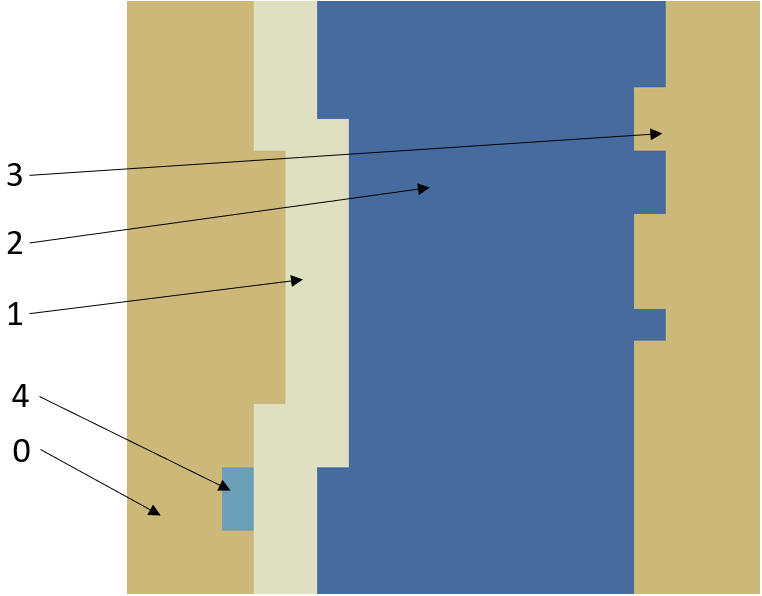
\includegraphics[width=\textwidth]{basic_landcover}
		\caption{Sample land cover}
		\label{Sample land cover}
	\end{subfigure}
	\vfill
	\begin{subfigure}[b]{.4\textwidth}
		\centering
		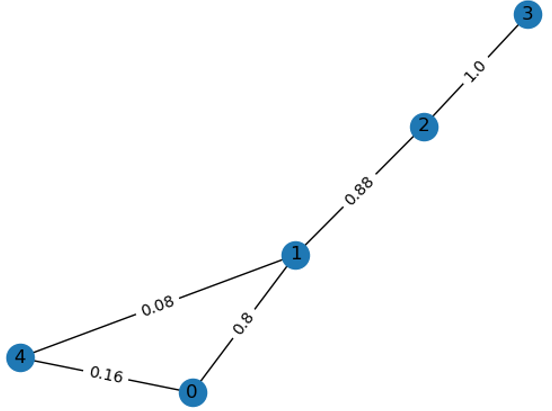
\includegraphics[width=\textwidth]{basic_landcover_graph}
		\caption{Resulting Graph}
		\label{Resulting Graph}
	\end{subfigure}
	\caption{This figure demonstrates how a section of land cover is converted into a graph. Each of the labeled sections of the image correspond to the node with the same label. The weights on the graph are the length of the shared perimeter relative to the length of the largest perimeter observed in the image which in this case is the one between 2 and 3.}
	\label{BasicTransform}
\end{figure}

With this representation new approaches can be used to compare vertices of the graph. In this paper we will be comparing three methods. These methods were selected due to their varying methodologies, optimization methods, and experimental performance. Basic details are given in TABLE \ref{NWRC}.

Each method produces vector embedding for each vertex of the graph. These vectors will be clustered using hierarchical clustering with ward linkage.

\renewcommand{\arraystretch}{1.2}
\begin{table*}[t]
	\begin{tabular}{|l|l|l|l|}
		\hline
		Method & Complexity      & Structure Captured     & Training Method                              \\
		\hline
		LINE   & $O(d|E|)$         & \multirow{2}{*}{Local} & \multirow{2}{*}{Stochastic Gradient Descent} \\
		\cline{1-2}
		LGAE   & $O(d|V|)$         &                        &                                              \\
		\hline
		GraRep & $O(|V||E|+d|V|2)$ & Global                 & Eigen Decomposition \\
		\hline
	\end{tabular}
	\caption{Comparison of basic attributes of the selected network representation methods}
	\label{NWRC}
\end{table*}
\renewcommand{\arraystretch}{1}

\subsection{Linear Graph Autoencoders \cite{SalhaGalvan2019KeepIS}}
An autoencoder is a model that is able to take data and convert it to a different representation of the data. Most of the time this new representation has reduced dimensionality or is able to represent the original data in a new format that is more conducive to other data mining tasks. The strength of an autoencoder is judged on its ability to recreate the input from the reduced form. A graph autoencoder is able to convert a vertex to a vector representation.

\subsection{GraRep \cite{Cao2015GraRepLG}}
GraRep creates a vector of step representations for each vertex on a graph. The ${k}$th value in the vector encodes information about graph ${k}$ steps from the vertex.

\subsection{LINE \cite{Tang2015LINELI}}
LINE creates vector representations for each vertex but unlike GraRep, the vector only represents a single  ${k}$ steps from the vertex.

\section{Proposed Research}
Further research needed to complete the project
How to handle very large and small regions?
Should node label data be introduced?

\subsection{Plan}
\begin{itemize}
\item Finish implementation of GraRep - 09 March 2022
\begin{itemize}
	\item Understand remaining parts mathematically of algorithm
	\item Create toy model to understand GraRep in a more overall sense
\end{itemize}
\item Perform runs with land cover classes combined into super classes 10 March 2022

\item Figure out how to handle very small regions - 12 March 2022
\begin{itemize}
	\item What is the threshold for a small region?
	\item Create method to determine what surrounding region to merge it into
\end{itemize}

\item Figure out how to handle very large regions - 14 March 2022
\begin{itemize}
	\item What is the threshold for a large region?
	\item What to do about disjoint graphs?
	\item Should they be left out of the final clustering?
\end{itemize}

\item Figure out if node labels should be used - 16 March 2022
\begin{itemize}
	\item What would benefits look like?
	\item How should they bee introduced into the pipeline?
	\item How should the "strength" of the node labels be in relation to the components found if labels are introduced after the components been found?
\end{itemize}

\item Finish implementation of Linear Graph Autoencoders - 09 March 2022
\begin{itemize}
	\item Understand the parts of the algorithm mathematically
	\item Create toy model to understand it in a more overall sense
\end{itemize}

\item Finish implementation of LINE - 09 March 2022
\begin{itemize}
	\item Understand the parts of the algorithm mathematically
	\item Create toy model to understand it in a more overall sense
\end{itemize}

\item Begin running tests on entire pipeline  - 09 March 2022

\end{itemize}


\section{Evaluation}
The resulting trees for each embedding algorithm can be split such that a desired number of regions are formed. Due to this fact as well as the methods being unsupervised means the resulting regions do not have any human defined meaning nor can the clusters be quantitative compared a ground truth. Therefore, the assessment will be based solely on the usefulness of the clusters. This will be done by examining the patterns found in each cluster qualitatively. The resulting clusters structure will also be compared to regions created by human conducted surveys.

\subsection {Results}
Example Result of Pipeline
\begin{itemize}
	\item Input image: 30x30 km region near New Orleans, LA
	\item Number of segments: 8096
	\item Network Representation Method used: GraRep
	\item GraRep Arguments:
	\begin{itemize}
		\item k=5
		\item d=5
	\end{itemize}
	\item Clustering Method: Hierarchical
	
\end{itemize}
Results can be viewed in Fig. \ref{Pipeline results}
\begin{figure*}[t!]
	\centering
	\begin{subfigure}[b]{0.4\textwidth}
		\centering
		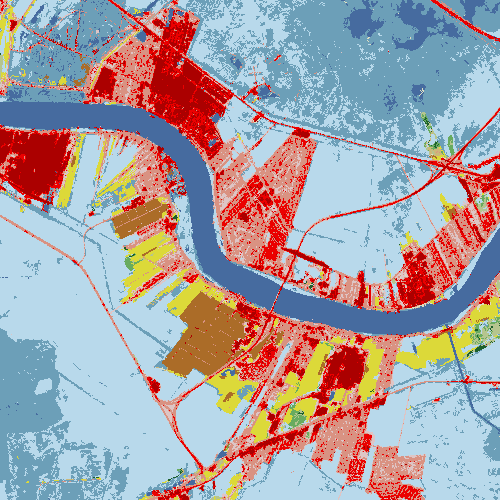
\includegraphics[width=\textwidth]{landcover}
		\caption{Land cover classes}
		\label{base}
	\end{subfigure}
	\hfill
	\begin{subfigure}[b]{0.4\textwidth}
		\centering
		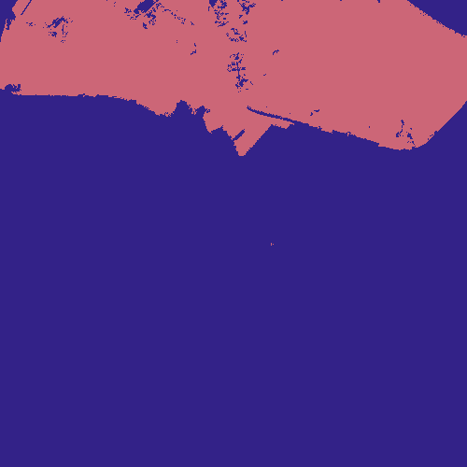
\includegraphics[width=\textwidth]{2clusters}
		\caption{2 clusters}
		\label{2 clusters}
	\end{subfigure}
	\hfill
	\begin{subfigure}[b]{0.4\textwidth}
		\centering
		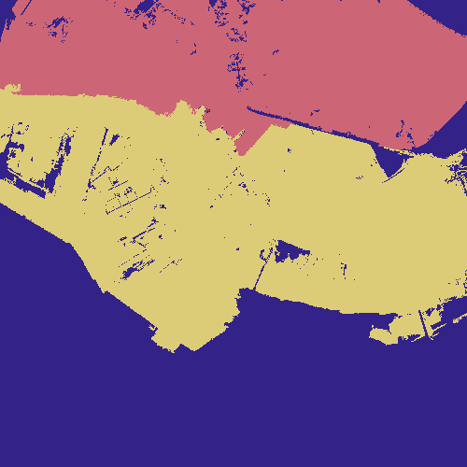
\includegraphics[width=\textwidth]{3clusters}
		\caption{3 clusters}
		\label{3 clusters}
	\end{subfigure}
	\hfill
	\begin{subfigure}[b]{0.4\textwidth}
		\centering
		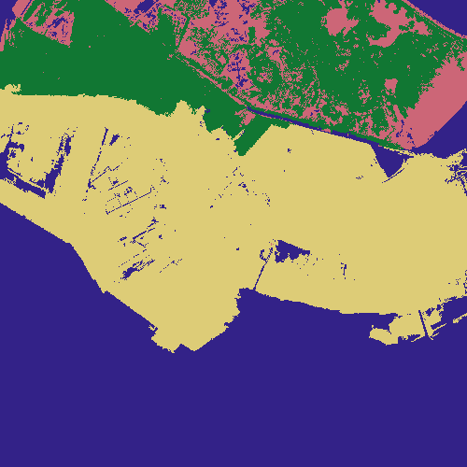
\includegraphics[width=\textwidth]{4clusters}
		\caption{4 clusters}
		\label{4 clusters}
	\end{subfigure}
	\caption{Pipeline results}
	\label{Pipeline results}
\end{figure*}
		


\section{Conclusion}

\bibliographystyle{IEEEtran}
\bibliography{./references}
	
	
\end{document}
